% Created by tikzDevice version 0.12
% !TEX encoding = UTF-8 Unicode
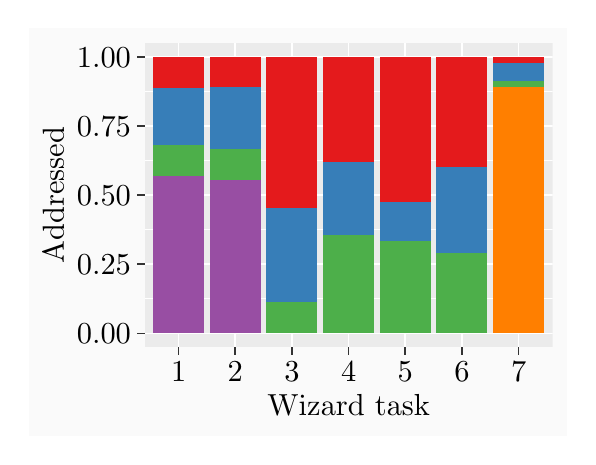
\begin{tikzpicture}[x=1pt,y=1pt]
\definecolor{fillColor}{RGB}{255,255,255}
\path[use as bounding box,fill=fillColor,fill opacity=0.00] (0,0) rectangle (195.19,147.70);
\begin{scope}
\path[clip] (  0.00,  0.00) rectangle (195.19,147.70);
\definecolor{drawColor}{RGB}{255,255,255}
\definecolor{fillColor}{gray}{0.98}

\path[draw=drawColor,line width= 0.6pt,line join=round,line cap=round,fill=fillColor] (  0.00, -0.00) rectangle (195.19,147.70);
\end{scope}
\begin{scope}
\path[clip] ( 42.27, 32.24) rectangle (189.69,142.20);
\definecolor{fillColor}{gray}{0.92}

\path[fill=fillColor] ( 42.27, 32.24) rectangle (189.69,142.20);
\definecolor{drawColor}{RGB}{255,255,255}

\path[draw=drawColor,line width= 0.3pt,line join=round] ( 42.27, 49.73) --
	(189.69, 49.73);

\path[draw=drawColor,line width= 0.3pt,line join=round] ( 42.27, 74.73) --
	(189.69, 74.73);

\path[draw=drawColor,line width= 0.3pt,line join=round] ( 42.27, 99.72) --
	(189.69, 99.72);

\path[draw=drawColor,line width= 0.3pt,line join=round] ( 42.27,124.71) --
	(189.69,124.71);

\path[draw=drawColor,line width= 0.6pt,line join=round] ( 42.27, 37.24) --
	(189.69, 37.24);

\path[draw=drawColor,line width= 0.6pt,line join=round] ( 42.27, 62.23) --
	(189.69, 62.23);

\path[draw=drawColor,line width= 0.6pt,line join=round] ( 42.27, 87.22) --
	(189.69, 87.22);

\path[draw=drawColor,line width= 0.6pt,line join=round] ( 42.27,112.21) --
	(189.69,112.21);

\path[draw=drawColor,line width= 0.6pt,line join=round] ( 42.27,137.21) --
	(189.69,137.21);

\path[draw=drawColor,line width= 0.6pt,line join=round] ( 54.56, 32.24) --
	( 54.56,142.20);

\path[draw=drawColor,line width= 0.6pt,line join=round] ( 75.03, 32.24) --
	( 75.03,142.20);

\path[draw=drawColor,line width= 0.6pt,line join=round] ( 95.50, 32.24) --
	( 95.50,142.20);

\path[draw=drawColor,line width= 0.6pt,line join=round] (115.98, 32.24) --
	(115.98,142.20);

\path[draw=drawColor,line width= 0.6pt,line join=round] (136.45, 32.24) --
	(136.45,142.20);

\path[draw=drawColor,line width= 0.6pt,line join=round] (156.93, 32.24) --
	(156.93,142.20);

\path[draw=drawColor,line width= 0.6pt,line join=round] (177.40, 32.24) --
	(177.40,142.20);
\definecolor{fillColor}{RGB}{152,78,163}

\path[fill=fillColor] ( 45.34, 37.24) rectangle ( 63.77, 94.04);
\definecolor{fillColor}{RGB}{77,175,74}

\path[fill=fillColor] ( 45.34, 94.04) rectangle ( 63.77,105.40);
\definecolor{fillColor}{RGB}{55,126,184}

\path[fill=fillColor] ( 45.34,105.40) rectangle ( 63.77,125.85);
\definecolor{fillColor}{RGB}{228,26,28}

\path[fill=fillColor] ( 45.34,125.85) rectangle ( 63.77,137.21);
\definecolor{fillColor}{RGB}{152,78,163}

\path[fill=fillColor] ( 65.82, 37.24) rectangle ( 84.24, 92.78);
\definecolor{fillColor}{RGB}{77,175,74}

\path[fill=fillColor] ( 65.82, 92.78) rectangle ( 84.24,103.88);
\definecolor{fillColor}{RGB}{55,126,184}

\path[fill=fillColor] ( 65.82,103.88) rectangle ( 84.24,126.10);
\definecolor{fillColor}{RGB}{228,26,28}

\path[fill=fillColor] ( 65.82,126.10) rectangle ( 84.24,137.21);
\definecolor{fillColor}{RGB}{77,175,74}

\path[fill=fillColor] ( 86.29, 37.24) rectangle (104.72, 48.60);
\definecolor{fillColor}{RGB}{55,126,184}

\path[fill=fillColor] ( 86.29, 48.60) rectangle (104.72, 82.68);
\definecolor{fillColor}{RGB}{228,26,28}

\path[fill=fillColor] ( 86.29, 82.68) rectangle (104.72,137.21);
\definecolor{fillColor}{RGB}{77,175,74}

\path[fill=fillColor] (106.76, 37.24) rectangle (125.19, 72.94);
\definecolor{fillColor}{RGB}{55,126,184}

\path[fill=fillColor] (106.76, 72.94) rectangle (125.19, 99.12);
\definecolor{fillColor}{RGB}{228,26,28}

\path[fill=fillColor] (106.76, 99.12) rectangle (125.19,137.21);
\definecolor{fillColor}{RGB}{77,175,74}

\path[fill=fillColor] (127.24, 37.24) rectangle (145.67, 70.56);
\definecolor{fillColor}{RGB}{55,126,184}

\path[fill=fillColor] (127.24, 70.56) rectangle (145.67, 84.84);
\definecolor{fillColor}{RGB}{228,26,28}

\path[fill=fillColor] (127.24, 84.84) rectangle (145.67,137.21);
\definecolor{fillColor}{RGB}{77,175,74}

\path[fill=fillColor] (147.71, 37.24) rectangle (166.14, 66.12);
\definecolor{fillColor}{RGB}{55,126,184}

\path[fill=fillColor] (147.71, 66.12) rectangle (166.14, 97.22);
\definecolor{fillColor}{RGB}{228,26,28}

\path[fill=fillColor] (147.71, 97.22) rectangle (166.14,137.21);
\definecolor{fillColor}{RGB}{255,127,0}

\path[fill=fillColor] (168.19, 37.24) rectangle (186.61,126.10);
\definecolor{fillColor}{RGB}{77,175,74}

\path[fill=fillColor] (168.19,126.10) rectangle (186.61,128.32);
\definecolor{fillColor}{RGB}{55,126,184}

\path[fill=fillColor] (168.19,128.32) rectangle (186.61,134.98);
\definecolor{fillColor}{RGB}{228,26,28}

\path[fill=fillColor] (168.19,134.98) rectangle (186.61,137.21);
\end{scope}
\begin{scope}
\path[clip] (  0.00,  0.00) rectangle (195.19,147.70);
\definecolor{drawColor}{RGB}{0,0,0}

\node[text=drawColor,anchor=base east,inner sep=0pt, outer sep=0pt, scale=  1.10] at ( 37.32, 33.45) {0.00};

\node[text=drawColor,anchor=base east,inner sep=0pt, outer sep=0pt, scale=  1.10] at ( 37.32, 58.44) {0.25};

\node[text=drawColor,anchor=base east,inner sep=0pt, outer sep=0pt, scale=  1.10] at ( 37.32, 83.43) {0.50};

\node[text=drawColor,anchor=base east,inner sep=0pt, outer sep=0pt, scale=  1.10] at ( 37.32,108.43) {0.75};

\node[text=drawColor,anchor=base east,inner sep=0pt, outer sep=0pt, scale=  1.10] at ( 37.32,133.42) {1.00};
\end{scope}
\begin{scope}
\path[clip] (  0.00,  0.00) rectangle (195.19,147.70);
\definecolor{drawColor}{gray}{0.20}

\path[draw=drawColor,line width= 0.6pt,line join=round] ( 39.52, 37.24) --
	( 42.27, 37.24);

\path[draw=drawColor,line width= 0.6pt,line join=round] ( 39.52, 62.23) --
	( 42.27, 62.23);

\path[draw=drawColor,line width= 0.6pt,line join=round] ( 39.52, 87.22) --
	( 42.27, 87.22);

\path[draw=drawColor,line width= 0.6pt,line join=round] ( 39.52,112.21) --
	( 42.27,112.21);

\path[draw=drawColor,line width= 0.6pt,line join=round] ( 39.52,137.21) --
	( 42.27,137.21);
\end{scope}
\begin{scope}
\path[clip] (  0.00,  0.00) rectangle (195.19,147.70);
\definecolor{drawColor}{gray}{0.20}

\path[draw=drawColor,line width= 0.6pt,line join=round] ( 54.56, 29.49) --
	( 54.56, 32.24);

\path[draw=drawColor,line width= 0.6pt,line join=round] ( 75.03, 29.49) --
	( 75.03, 32.24);

\path[draw=drawColor,line width= 0.6pt,line join=round] ( 95.50, 29.49) --
	( 95.50, 32.24);

\path[draw=drawColor,line width= 0.6pt,line join=round] (115.98, 29.49) --
	(115.98, 32.24);

\path[draw=drawColor,line width= 0.6pt,line join=round] (136.45, 29.49) --
	(136.45, 32.24);

\path[draw=drawColor,line width= 0.6pt,line join=round] (156.93, 29.49) --
	(156.93, 32.24);

\path[draw=drawColor,line width= 0.6pt,line join=round] (177.40, 29.49) --
	(177.40, 32.24);
\end{scope}
\begin{scope}
\path[clip] (  0.00,  0.00) rectangle (195.19,147.70);
\definecolor{drawColor}{RGB}{0,0,0}

\node[text=drawColor,anchor=base,inner sep=0pt, outer sep=0pt, scale=  1.10] at ( 54.56, 19.71) {1};

\node[text=drawColor,anchor=base,inner sep=0pt, outer sep=0pt, scale=  1.10] at ( 75.03, 19.71) {2};

\node[text=drawColor,anchor=base,inner sep=0pt, outer sep=0pt, scale=  1.10] at ( 95.50, 19.71) {3};

\node[text=drawColor,anchor=base,inner sep=0pt, outer sep=0pt, scale=  1.10] at (115.98, 19.71) {4};

\node[text=drawColor,anchor=base,inner sep=0pt, outer sep=0pt, scale=  1.10] at (136.45, 19.71) {5};

\node[text=drawColor,anchor=base,inner sep=0pt, outer sep=0pt, scale=  1.10] at (156.93, 19.71) {6};

\node[text=drawColor,anchor=base,inner sep=0pt, outer sep=0pt, scale=  1.10] at (177.40, 19.71) {7};
\end{scope}
\begin{scope}
\path[clip] (  0.00,  0.00) rectangle (195.19,147.70);
\definecolor{drawColor}{RGB}{0,0,0}

\node[text=drawColor,anchor=base,inner sep=0pt, outer sep=0pt, scale=  1.10] at (115.98,  7.44) {Wizard task};
\end{scope}
\begin{scope}
\path[clip] (  0.00,  0.00) rectangle (195.19,147.70);
\definecolor{drawColor}{RGB}{0,0,0}

\node[text=drawColor,rotate= 90.00,anchor=base,inner sep=0pt, outer sep=0pt, scale=  1.10] at ( 13.08, 87.22) {Addressed};
\end{scope}
\end{tikzpicture}
